\FloatBarrier
\clearpage
\section{External-Family Density Controls}
\label{app:external-density-controls}
These two archived comparisons characterize generic density estimators on
classical and copula distributions. Each uses five repetitions with 1000
training and 1000 independent test observations per scenario. Oracle rows
evaluate the known generating density; neither comparison fits an SFD.
The full score and summary tables accompany the compilation sources.
Finite scores from runs with iteration-limit warnings remain in the means;
the archived status columns identify those runs.

\begin{figure}[H]
\centering
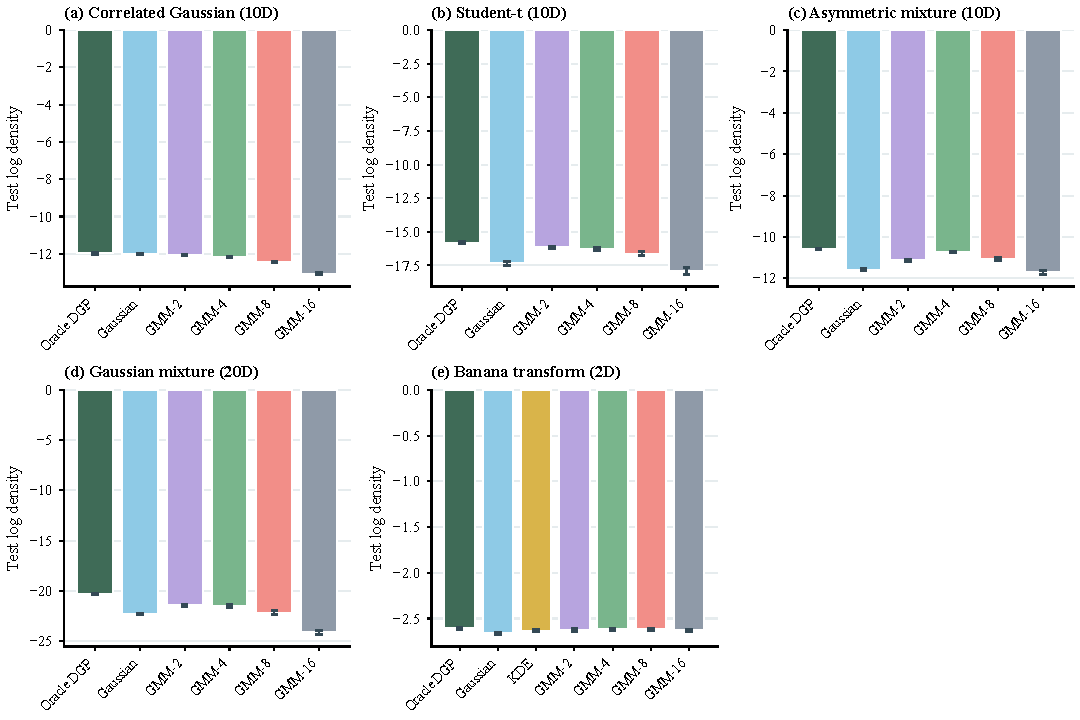
\includegraphics[width=\linewidth,clip]{figures/classical_density_controls.pdf}
\caption{Classical distributions: correlated Gaussian, Student-$t$,
asymmetric Gaussian mixture, Gaussian mixture and banana transform.
Bars show mean test log density and one Monte Carlo SE over five
repetitions. The oracle is the generating density; no SFD is fitted.}
\label{fig:classical-controls}
\end{figure}

\paragraph{Classical-family settings.}
The first three distributions have ten coordinates, the Gaussian mixture
has twenty, and the banana transform has two. GMM sizes are $2,4,8,16$,
with maximum 50 iterations, tolerance $10^{-5}$ and covariance
regularization $10^{-5}$. KDE is included only for the two-dimensional
scenario. The base seed is 20260624. These reduced-scale controls are
separate from the 25-repetition known-skeleton diagnostic.

\clearpage
\paragraph{Copula-family settings.}
The Gaussian and Student-$t$ copulas have ten coordinates; Clayton has five.
The Gaussian correlation is $0.55$. The Student-$t$ copula has correlation
$0.45$ and $4.5$ degrees of freedom. The Clayton parameter is $1.6$.
GMM sizes are $2,4,8,16$, with maximum 60 iterations, tolerance $10^{-5}$
and covariance regularization $10^{-5}$; KDE is included for Clayton only.
The base seed is 20260624. These controls do not include a fitted vine copula.

\begin{figure}[H]
\centering
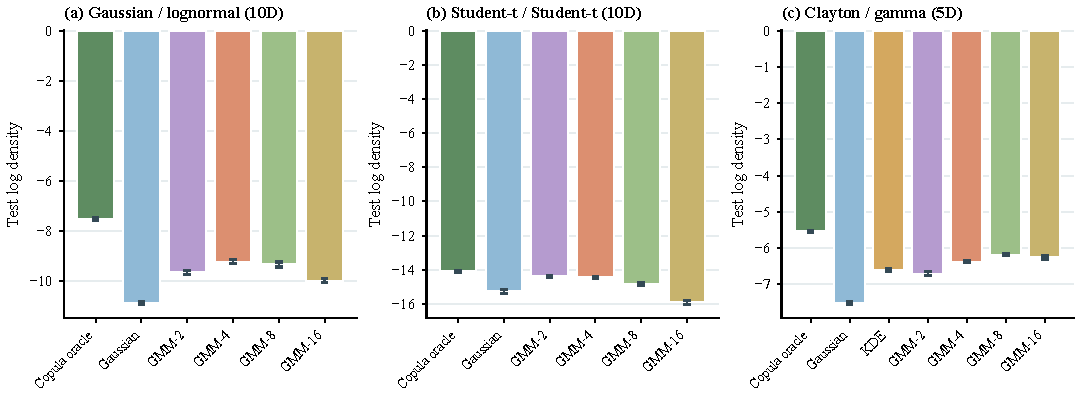
\includegraphics[width=\linewidth,clip]{figures/copula_density_controls.pdf}
\caption{Copula families: Gaussian with lognormal margins, Student-$t$
with Student-$t$ margins, and Clayton with gamma margins. Bars show mean
test log density and one Monte Carlo SE over five repetitions. The oracle
includes the copula and marginal densities; no SFD is fitted.}
\label{fig:copula-controls}
\end{figure}
\FloatBarrier
